\part{Introduction}

\section{Introduction}

\subsection{Background}

\begin{frame}
  \frametitle{Motivation}

  \begin{block}<1->{The Rise of Big Data}
    \begin{itemize}
      \item Modern applications generate vast quantities of data
      \item Exponential growth of data
      \item Difficult to store and process
      \item Data generation is increasing at a greater rate than data storage
    \end{itemize}
  \end{block}

  \begin{block}<2->{Example}
    \begin{itemize}
      \item Very Large Array collects hundreds of terabytes annually
      \item Square Kilometre Array will store two petabytes daily
    \end{itemize}
  \end{block}
\end{frame}

\begin{frame}
  \frametitle{Solution}

  \begin{block}<1->{Streaming Algorithms}
    \begin{itemize}
      \item Streams of arbitrary length and order
      \item One item at a time
      \item Compact summaries of data
      \begin{itemize}
        \item A handful of values
        \item A reduced array or `sketch'
      \end{itemize}
      \item Approximations of properties of data
    \end{itemize}
  \end{block}

  \begin{block}<2->{Advantages}
    \begin{itemize}
      \item Reduced size
      \item Efficient queries
      \item Ease of update
    \end{itemize}
  \end{block}
\end{frame}

\begin{frame}
  \frametitle{Applications}

  \begin{block}<1->{Characteristics}
    \begin{itemize}
      \item Large and constantly changing data
      \item Data locality
      \item Approximate results
    \end{itemize}
  \end{block}

  \begin{block}<2->{Examples}
    \begin{itemize}
      \item Medicine
      \item Science
      \item Business
      \item Social media
    \end{itemize}
  \end{block}
\end{frame}

\subsection{Aims and Objectives}

\begin{frame}
  \frametitle{Overview}

  \begin{block}<1->{Aims}
    \begin{itemize}
      \item Investigate streaming algorithms and their applications
      \item Implement the fingerprint summary, count sketch and dyadic count sketch from scratch to create a small library in Java
    \end{itemize}
  \end{block}

  \begin{block}<2->{Objectives}
    \begin{itemize}
      \item Understand theoretically
      \item Express formally in pseudocode
      \item Analyse correctness, complexity and advantages
      \item Implemented in Java
      \item Evaluated on datasets
    \end{itemize}
  \end{block}

\end{frame}

\begin{frame}
  \frametitle{Summaries}

  \begin{block}<1->{Multiset Data}
    \begin{itemize}
      \item Pairs of items and weights
      \item Useful for mapped data
      \item Streaming model allows insertion and deletion
    \end{itemize}
  \end{block}

  \begin{block}<2->{Multiset Summaries}
    \begin{itemize}
      \item<2-> Fingerprint summary---identification
      \item<3-> Count sketch---frequencies
      \item<4-> Dyadic count sketch---ranks and quantiles
    \end{itemize}
  \end{block}
\end{frame}

\subsection{Structure and Contributions}

\begin{frame}
  \frametitle{The Implementation Library}

  \begin{adjustbox}{
    max height = \textheight,
    max width = \textwidth,
  }
    \definecolor{plantucolor0000}{RGB}{254,254,206}
\definecolor{plantucolor0001}{RGB}{168,0,54}
\definecolor{plantucolor0002}{RGB}{180,167,229}
\definecolor{plantucolor0003}{RGB}{0,0,0}
\definecolor{plantucolor0004}{RGB}{132,190,132}
\definecolor{plantucolor0005}{RGB}{3,128,72}
\definecolor{plantucolor0006}{RGB}{173,209,178}

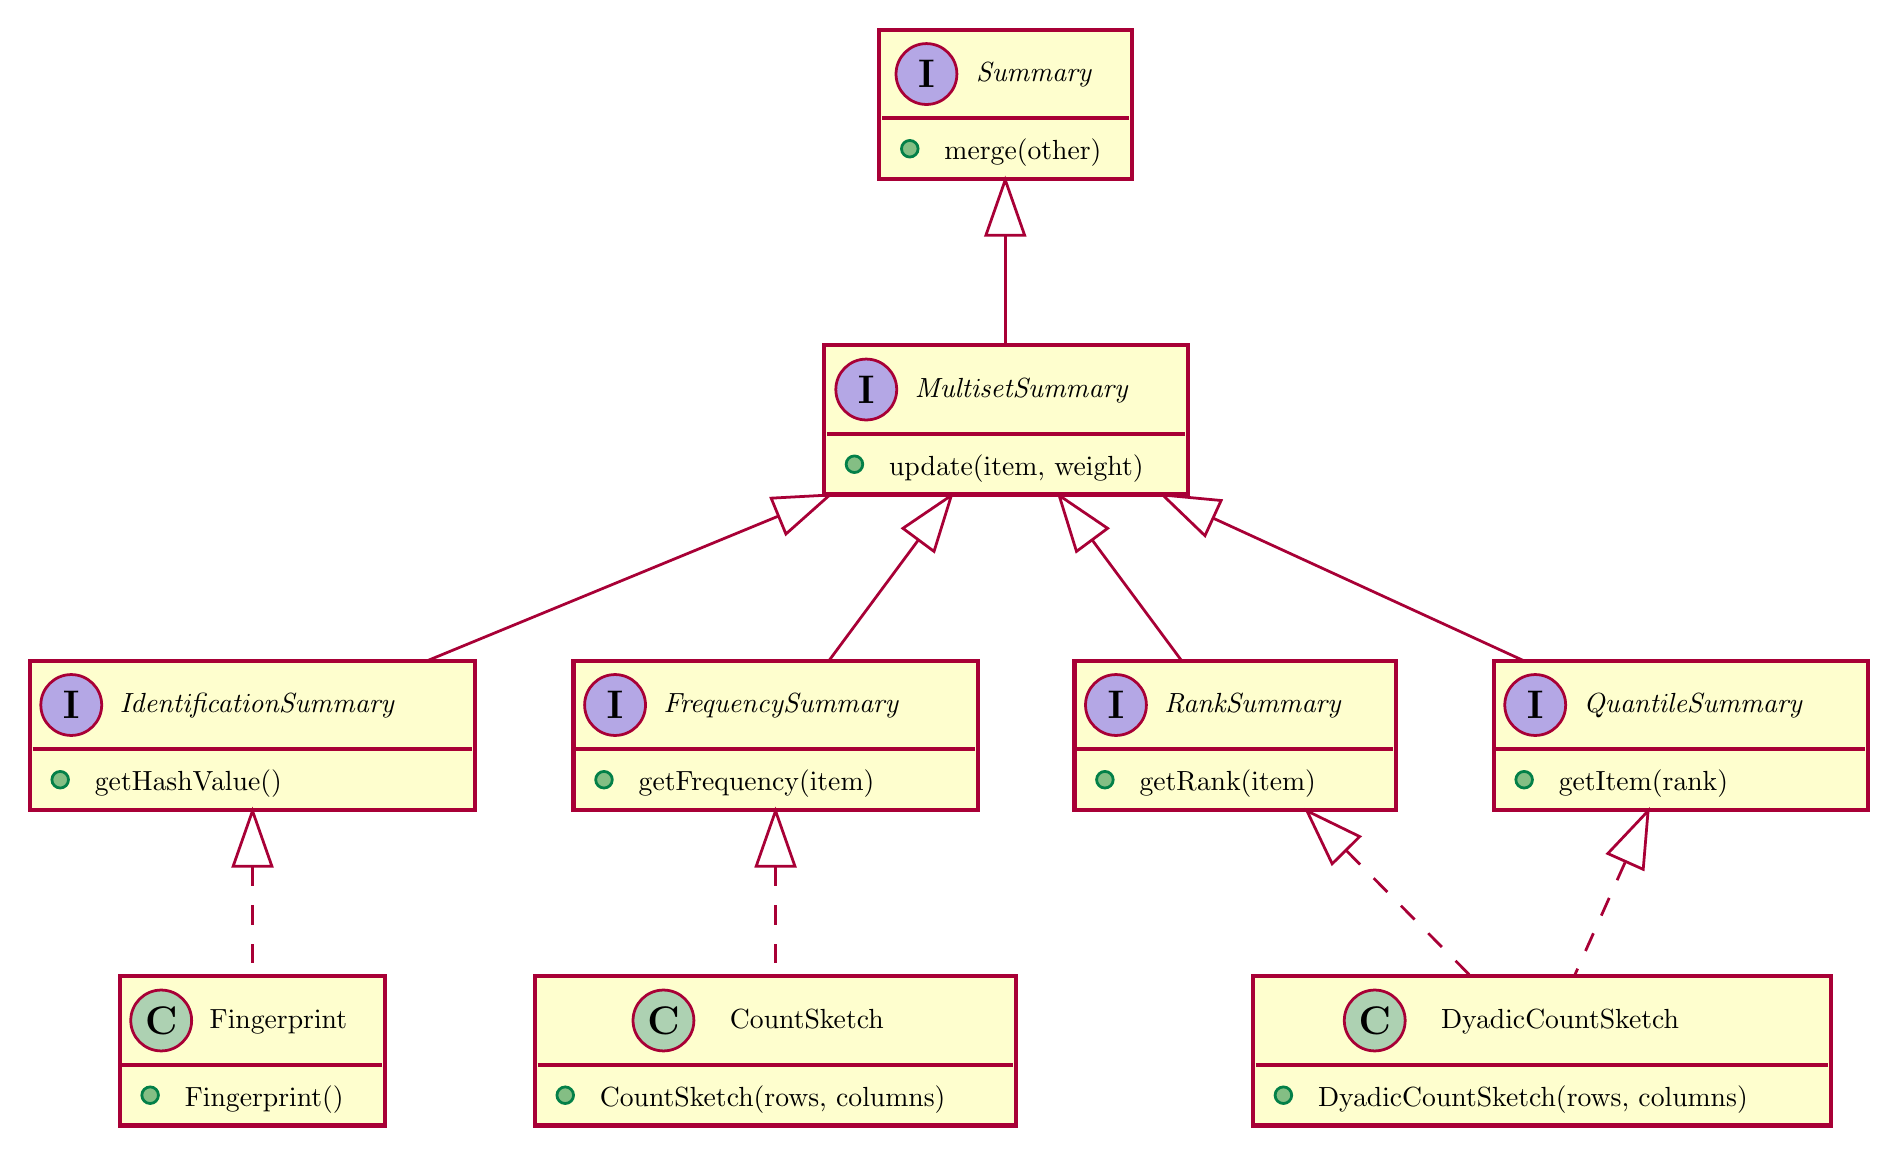
\begin{tikzpicture}[
  yscale=-1,
  pstyle0/.style={color=plantucolor0001,fill=plantucolor0000,line width=1.5pt},
  pstyle1/.style={color=plantucolor0001,fill=plantucolor0002,line width=1.0pt},
  pstyle2/.style={color=plantucolor0001,line width=1.5pt},
  pstyle3/.style={color=plantucolor0005,fill=plantucolor0004,line width=1.0pt},
  pstyle4/.style={color=plantucolor0001,fill=plantucolor0006,line width=1.0pt},
  pstyle5/.style={color=plantucolor0001,line width=1.0pt},
  pstyle6/.style={color=plantucolor0001,line width=1.0pt,dash pattern=on 7.0pt off 7.0pt},
]
  \action<2->{
    \draw[pstyle0] (314pt,7pt) rectangle (405.2656pt,60.9434pt);
    \draw[pstyle1] (331.0252pt,23pt) ellipse (11pt and 11pt);
    \node at (331.0252pt,23pt)[]{\textbf{\Large I}};
    \node at (345.4752pt,15.3945pt)[below right,color=black]{\textit{Summary}};
    \draw[pstyle2] (315pt,39pt) -- (404.2656pt,39pt);
    \draw[pstyle3] (325pt,50pt) ellipse (3pt and 3pt);
    \node at (334pt,43pt)[below right,color=black]{merge(other)};
  }
  \action<3->{
    \draw[pstyle0] (294pt,121pt) rectangle (425.4105pt,174.9434pt);
    \draw[pstyle1] (309.2747pt,137pt) ellipse (11pt and 11pt);
    \node at (309.2747pt,137pt)[]{\textbf{\Large I}};
    \node at (323.3358pt,129.3945pt)[below right,color=black]{\textit{MultisetSummary}};
    \draw[pstyle2] (295pt,153pt) -- (424.4105pt,153pt);
    \draw[pstyle3] (305pt,164pt) ellipse (3pt and 3pt);
    \node at (314pt,157pt)[below right,color=black]{update(item, weight)};
  }
  \action<4->{
    \draw[pstyle0] (7pt,235pt) rectangle (167.9704pt,288.9434pt);
    \draw[pstyle1] (22pt,251pt) ellipse (11pt and 11pt);
    \node at (22pt,251pt)[]{\textbf{\Large I}};
    \node at (36pt,243.3945pt)[below right,color=black]{\textit{IdentificationSummary}};
    \draw[pstyle2] (8pt,267pt) -- (166.9704pt,267pt);
    \draw[pstyle3] (18pt,278pt) ellipse (3pt and 3pt);
    \node at (27pt,271pt)[below right,color=black]{getHashValue()};
    \draw[pstyle0] (203.5pt,235pt) rectangle (349.5333pt,288.9434pt);
    \draw[pstyle1] (218.5pt,251pt) ellipse (11pt and 11pt);
    \node at (218.5pt,251pt)[]{\textbf{\Large I}};
    \node at (232.5pt,243.3945pt)[below right,color=black]{\textit{FrequencySummary}};
    \draw[pstyle2] (204.5pt,267pt) -- (348.5333pt,267pt);
    \draw[pstyle3] (214.5pt,278pt) ellipse (3pt and 3pt);
    \node at (223.5pt,271pt)[below right,color=black]{getFrequency(item)};
    \draw[pstyle0] (384.5pt,235pt) rectangle (500.5732pt,288.9434pt);
    \draw[pstyle1] (399.5pt,251pt) ellipse (11pt and 11pt);
    \node at (399.5pt,251pt)[]{\textbf{\Large I}};
    \node at (413.5pt,243.3945pt)[below right,color=black]{\textit{RankSummary}};
    \draw[pstyle2] (385.5pt,267pt) -- (499.5732pt,267pt);
    \draw[pstyle3] (395.5pt,278pt) ellipse (3pt and 3pt);
    \node at (404.5pt,271pt)[below right,color=black]{getRank(item)};
    \draw[pstyle0] (536pt,235pt) rectangle (671.2046pt,288.9434pt);
    \draw[pstyle1] (551pt,251pt) ellipse (11pt and 11pt);
    \node at (551pt,251pt)[]{\textbf{\Large I}};
    \node at (565pt,243.3945pt)[below right,color=black]{\textit{QuantileSummary}};
    \draw[pstyle2] (537pt,267pt) -- (670.2046pt,267pt);
    \draw[pstyle3] (547pt,278pt) ellipse (3pt and 3pt);
    \node at (556pt,271pt)[below right,color=black]{getItem(rank)};
  }
  \action<5->{
    \draw[pstyle0] (39.5pt,349pt) rectangle (135.263pt,402.9434pt);
    \draw[pstyle4] (54.5pt,365pt) ellipse (11pt and 11pt);
    \node at (54.5pt,365pt)[]{\textbf{\Large C}};
    \node at (68.5pt,357.3945pt)[below right,color=black]{Fingerprint};
    \draw[pstyle2] (40.5pt,381pt) -- (134.263pt,381pt);
    \draw[pstyle3] (50.5pt,392pt) ellipse (3pt and 3pt);
    \node at (59.5pt,385pt)[below right,color=black]{Fingerprint()};
    \draw[pstyle0] (189.5pt,349pt) rectangle (363.4455pt,402.9434pt);
    \draw[pstyle4] (235.9905pt,365pt) ellipse (11pt and 11pt);
    \node at (235.9905pt,365pt)[]{\textbf{\Large C}};
    \node at (256.4905pt,357.3945pt)[below right,color=black]{CountSketch};
    \draw[pstyle2] (190.5pt,381pt) -- (362.4455pt,381pt);
    \draw[pstyle3] (200.5pt,392pt) ellipse (3pt and 3pt);
    \node at (209.5pt,385pt)[below right,color=black]{CountSketch(rows, columns)};
    \draw[pstyle0] (449pt,349pt) rectangle (657.8976pt,402.9434pt);
    \draw[pstyle4] (493.0053pt,365pt) ellipse (11pt and 11pt);
    \node at (493.0053pt,365pt)[]{\textbf{\Large C}};
    \node at (513.451pt,357.3945pt)[below right,color=black]{DyadicCountSketch};
    \draw[pstyle2] (450pt,381pt) -- (656.8976pt,381pt);
    \draw[pstyle3] (460pt,392pt) ellipse (3pt and 3pt);
    \node at (469pt,385pt)[below right,color=black]{DyadicCountSketch(rows, columns)};
  }
  \action<3->{
    \draw[pstyle5] (359.5pt,81.37pt) ..controls (359.5pt,94.87pt) and (359.5pt,109.13pt) .. (359.5pt,120.91pt);
    \draw[pstyle5] (352.5pt,81.26pt) -- (359.5pt,61.26pt) -- (366.5pt,81.26pt) -- (352.5pt,81.26pt) -- cycle;
  }
  \action<4->{
    \draw[pstyle5] (277.45pt,182.78pt) ..controls (236.91pt,199.48pt) and (188.72pt,219.32pt) .. (151.03pt,234.84pt);
    \draw[pstyle5] (274.91pt,176.26pt) -- (296.07pt,175.12pt) -- (280.24pt,189.21pt) -- (274.91pt,176.26pt) -- cycle;
    \draw[pstyle5] (327.98pt,191.53pt) ..controls (317.17pt,206.12pt) and (305.39pt,222.01pt) .. (295.84pt,234.91pt);
    \draw[pstyle5] (322.51pt,187.16pt) -- (340.04pt,175.26pt) -- (333.76pt,195.5pt) -- (322.51pt,187.16pt) -- cycle;
    \draw[pstyle5] (391.02pt,191.53pt) ..controls (401.83pt,206.12pt) and (413.61pt,222.01pt) .. (423.16pt,234.91pt);
    \draw[pstyle5] (385.24pt,195.5pt) -- (378.96pt,175.26pt) -- (396.49pt,187.16pt) -- (385.24pt,195.5pt) -- cycle;
    \draw[pstyle5] (434.59pt,183.47pt) ..controls (470.65pt,200.02pt) and (513.16pt,219.53pt) .. (546.51pt,234.84pt);
    \draw[pstyle5] (431.66pt,189.82pt) -- (416.4pt,175.12pt) -- (437.5pt,177.1pt) -- (431.66pt,189.82pt) -- cycle;
  }
  \action<5->{
    \draw[pstyle6] (87.5pt,309.37pt) ..controls (87.5pt,322.87pt) and (87.5pt,337.13pt) .. (87.5pt,348.91pt);
    \draw[pstyle5] (80.5pt,309.26pt) -- (87.5pt,289.26pt) -- (94.5pt,309.26pt) -- (80.5pt,309.26pt) -- cycle;
    \draw[pstyle6] (276.5pt,309.37pt) ..controls (276.5pt,322.87pt) and (276.5pt,337.13pt) .. (276.5pt,348.91pt);
    \draw[pstyle5] (269.5pt,309.26pt) -- (276.5pt,289.26pt) -- (283.5pt,309.26pt) -- (269.5pt,309.26pt) -- cycle;
    \draw[pstyle6] (482.78pt,303.64pt) ..controls (497.74pt,318.74pt) and (514.3pt,335.45pt) .. (527.64pt,348.91pt);
    \draw[pstyle5] (477.63pt,308.39pt) -- (468.52pt,289.26pt) -- (487.58pt,298.54pt) -- (477.63pt,308.39pt) -- cycle;
    \draw[pstyle6] (583.44pt,307.92pt) ..controls (577.23pt,321.84pt) and (570.59pt,336.71pt) .. (565.15pt,348.91pt);
    \draw[pstyle5] (577.23pt,304.67pt) -- (591.78pt,289.26pt) -- (590.02pt,310.38pt) -- (577.23pt,304.67pt) -- cycle;
  }
\end{tikzpicture}

  \end{adjustbox}
\end{frame}

\begin{frame}
  \frametitle{The Written Work}

  \begin{block}<1->{Understanding of streaming algorithms}
    \begin{itemize}
      \item Applications
      \item Theory
      \item Analysis of correctness
      \item Empirical verification of analyses
    \end{itemize}
  \end{block}

  \begin{block}<2->{Further Contributions}
    \begin{itemize}
      \item More digestible as introductory material
      \item Original analyses
      \begin{itemize}
        \item Comparison to traditional methods
        \item Extending the universe of permissible values
      \end{itemize}
    \end{itemize}
  \end{block}
\end{frame}

\begin{frame}
  \frametitle{This Presentation}

  \begin{block}{Summaries}
    \begin{itemize}
      \item Overview
      \item Applications
      \item Algorithms
      \item Analysis of correctness
    \end{itemize}
  \end{block}
\end{frame}
